% fig_oc_fault_levels.tex
% TR-40: Fault level comparison — grid-connected vs islanded
%
% Grouped bar chart:
%   Group 1: Mid-line fault (GC=22.22 pu, IS=8.00 pu)
%   Group 2: Far-end fault  (GC=14.29 pu, IS=4.00 pu)
%
% Values normalised to rated IBR current (1.0 pu)

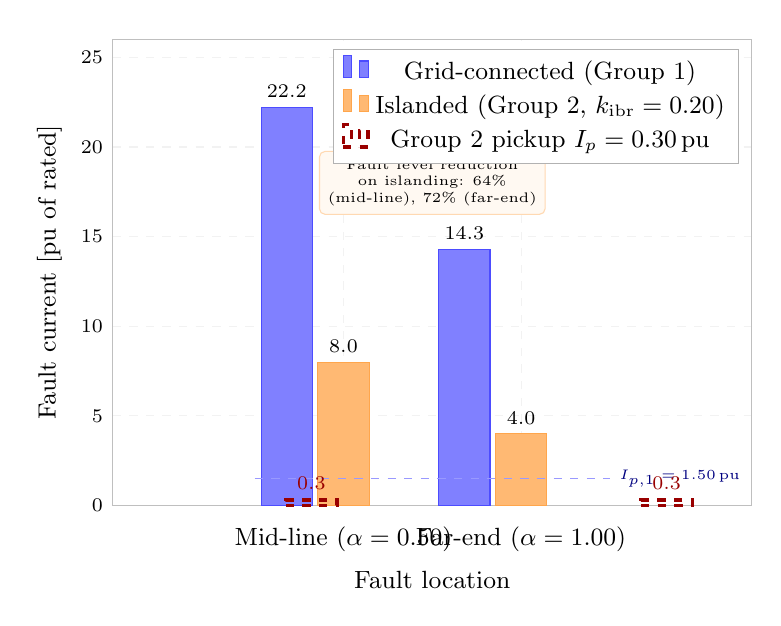
\begin{tikzpicture}
\begin{axis}[
  name         = flax,
  width        = 0.80\textwidth,
  height       = 7.5cm,
  ybar,
  bar width    = 0.65cm,
  xlabel       = {Fault location},
  ylabel       = {Fault current [pu of rated]},
  xlabel style = {font=\small},
  ylabel style = {font=\small},
  ymin=0, ymax=26,
  ytick        = {0,5,10,15,20,25},
  yticklabel style={font=\scriptsize},
  xtick        = {1,2},
  xticklabels  = {Mid-line ($\alpha=0.50$),
                  Far-end ($\alpha=1.00$)},
  xticklabel style={font=\small},
  tick style   = {draw=none},
  axis line style={gray!50},
  grid         = major,
  grid style   = {gray!10, dashed},
  nodes near coords,
  nodes near coords style={font=\scriptsize, anchor=south},
  every node near coord/.append style={
    /pgf/number format/.cd, fixed, fixed zerofill, precision=1
  },
  legend style={at={(0.98,0.98)}, anchor=north east, font=\small,
                draw=gray!60, fill=white},
  enlarge x limits=0.40,
  clip=false,
]

%% Grid-connected fault level
\addplot[fill=blue!50, draw=blue!70]
  coordinates {(1,22.2) (2,14.3)};
\addlegendentry{Grid-connected (Group 1)}

%% Islanded fault level
\addplot[fill=orange!55, draw=orange!70]
  coordinates {(1,8.0) (2,4.0)};
\addlegendentry{Islanded (Group 2, $k_\mathrm{ibr}=0.20$)}

%% Group 2 pickup line
\addplot[red!60!black, very thick, dashed, mark=none]
  coordinates {(0.5, 0.30) (2.5, 0.30)};
\addlegendentry{Group 2 pickup $I_p=0.30$\,pu}

%% Reduction annotation
\node[draw=orange!30, fill=orange!5, rounded corners=2pt,
      font=\tiny, inner sep=3pt, align=center]
  at (axis cs:1.5, 18)
  {Fault level reduction\\on islanding: 64\%\\
   (mid-line), 72\% (far-end)};

%% Group 1 pickup line (invisible but reference)
\draw[blue!40, thin, dashed]
  (axis cs:0.5, 1.50) -- (axis cs:2.5, 1.50);
\node[blue!50!black, font=\tiny, right] at (axis cs:2.5, 1.50)
  {$I_{p,1}=1.50$\,pu};

\end{axis}
\end{tikzpicture}
